\subsection{Séptimo \textit{Sprint Huddle} de Producción} 
Tal como se indicó en el sexto sprint, la siguiente tarea que se ejecutó una 
vez terminados los sprites y las maquetas de los niveles, fue la programación de 
las clases actoras. 

\subsubsection{Implementando los enemigos normales del juego} 
Las primeras clases actoras en ser programadas fueron las correspondientes a los 
enemigos normales, estas clases se programaron a la par que la clase \textit{Player}. 
Si bien la clase \textit{Player} ya estaba programada desde los primeros prototipos, 
esta clase no contaba con toda su funcionalidad implementada y la funcionalidad 
faltante tuvo que ser implementada a la par que otras clases para verificar el 
correcto funcionamiento en la interacción de clases como la de los enemigos y los 
\textit{items}.
\\
\par 
Es verdad que ya existían enemigos desde los primeros prototipos; no obstante, 
su funcionalidad tuvo que ser reimplementada a fin de ofrecer un desempeño que 
optimizará recursos y agregará nuevas funcionalidades. A continuación, se listan los 
cambios que presentan los enemigos de séptimo \textit{sprint} en relación de los 
enemigos del primer prototipo: 

	\begin{itemize}
		 \item \textbf{Áreas de acción}: En el primer prototipo los enemigos ejecutaban 
		 sus patrones de movimiento y ataque sin importar que éstos se encontraran 
		 visibles para el jugador o no. Los enemigos del séptimo \textit{sprint} 
		 cuentan con áreas de acción definida, lo que hace que sus patrones de 
		 movimientos y ataques solo se ejecuten si el jugador entra a estas áreas 
		 activas. Esto permite que el dispositivo no gaste recursos en objetos que no se 
		 encuentran visible para el jugador (ver figura ).
		 \begin{figure}[h]
    			\centering
    			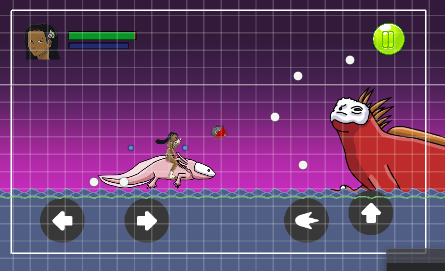
\includegraphics[width=0.6\textwidth]{05TrabajoReali/imagenes/tilemaps01.png}
    			\caption{Vista de la escena cuando se tiene un \textit{GameObject} de 
    			tipo \textit{Tilemaps} para la construcción de niveles}
    			\label{fig:EnemyArea}
			\end{figure}
		   
Cantidad de vida: En el primer prototipo todos los enemigos eran derrotados por un único disparo, esto limitaba el factor de reto del juego al no ofrecer enemigos más resistentes al ataque del jugador. En el fin de ofrecer una nueva capa de complejidad a los enemigos se agregó a la clase Enemy el atributo maxHealth y healthAmount, estos atributos serían los encargados de almacenar la máxima cantidad de vida que un enemigo puede tener y la vida actual de dicho enemigo. La cantidad de vida sólo se actualizaría cuando el enemigo fuera atacado por el jugador o cuando se reiniciara el nivel. Para la actualización de la vida del enemigo se utilizó el comando Clamp de la clase Math, este comando permite especificar rangos con valores máximos y mínimos del resultado de operaciones, esto con la finalidad de que la vida actual del enemigo nunca sea cero y nunca sobrepase a su máximo de vida.
Cantidad de daño: Al igual que con la cantidad de vida, los enemigos del primer prototipo inflingian la misma cantidad de daño sin importar su tipo; por lo que para tener enemigos más y menos fuertes se agregó el atributo damageAmount. Un enemigo puede infringir daño al jugado cada vez que toca al jugador o cuando dispara un ataque. Cada vez que un enemigo o un disparo enemigo choca con el jugador, el objeto enemigo manda a llamar el método SetHealth del Player y le envía como parámetro el valor de su atributo damageAmount, seguido de un segundo método de la clase player llamado EnemyNockBack, este método es el encargado de la animación que indica que el jugador ha recibido daño.
 Girar horizontalmente: En el primer prototipo el enemigo era incapaz de girar sus Sprite y su ataque una vez que el jugador lo sobrepasaba como se ve en la figura (). Utilizando la posición del enemigo y la posición del jugador dentro del área activa, el enemigo puede voltear si sprite y su ataque   con base al valor de la distancia entre este y el jugador: Si es menor a  1 el enemigo mantiene su orientación inicial, si es mayor a 1 el enemigo se voltea. Voltear un Sprite no representa mayor problema en código; sin embargo, el voltear un sprite cuyo colisionador no seas simétrico como el de la figura puede representar un problema cuando tiene que detectar colisiones, tal y como ocurre con los enemigos de tipo RedGost y PulpleGost; para evitar alterar la detección de colisiones se creó una nueva clase auxiliar llamada FixerCollider,  cuyo objetivo es ajustar la posición del colisionador una vez que el personaje se gira como se puede observar en la figura ().
Trigger Collider: En el primer prototipo el colisionador del enemigo tenía una configuración del tipo sólido lo que ocasionaba que cuando el enemigo chocara con otro enemigo o con algún ataque enemigo este se estancara o fuera empujado por el objeto contra el que chocaba (ver figura ). Para corregir este comportamiento se configuro el colisionador como uno de tipo trigger (ver figura ).  
Rigidbody2D: Para evitar el comportamiento mencionado en el Trigger Collider también fue necesario modificar la configuración del componente Rigidbody2D, este componente paso de estar en modo Dynamic a modo Kinematic lo que permite evitar que el objeto de juego reaccione conforme a las leyes físicas comunes.   
Para implementar cada uno de los patrones de movimiento de los enemigos fue necesario utilizar posiciones auxiliares que indicaran el límite del movimiento del personaje, salvo en la clase Vulture ya que este explota al hacer contacto con el jugador.
Para resaltar la muerte de un enemigo se agregó un efecto especial de explosión acompañado de un efecto de sonido para la explosión del personaje. Para esta funcionalidad se implementó la clase SFXCtrl y AudioCtrl para manejar los efectos de especiales y el sonido respectivamente.
	\end{itemize}

Implementando los enemigos jefes del juego.
Para la implementación de los jefes se reutilizo las configuraciones de los enemigos normales referente a componentes como Rigidbody2D y el Colisionador, el uso de la clase Enemy para el manejo de vida y el uso de los efectos de sonido y de explosiones para la muerte del jefe.
La lógica, al menos en la teoría, tras los jefes del juego fue inspirada por el jefe Roxas (ver figura ) del juego Kingdom Hearts 2 Final Mix. Dentro de Kingdom Hearts 2 Final Mix, Roxas es uno de los jefes que requiere mayor habilidad de juego para ser derrotado, ya que a diferencia del resto de los jefes del Kingdom Hearts 2 Final Mix, el patrón de ataque de Roxas era totalmente aleatorio; el jugador podía saber en qué consistía cada uno de los ataques de este jefe, pero desconocía el orden en el que estos serían ejecutados, salvo por algunos ataques que estaban condicionados a una secuencia de ataque anterior.  Con los jefes del juego Yolotl sucede algo parecido, el jugador puede llegar a conocer lo tipos de ataque que posee un jefe determinado pero la secuencia de ejecución de los ataques está programada para que sea aleatoria, lo que puede generar experiencias de juego muy sencillas o bastante retadoras para el jugador. El anterior comportamiento se logra simulando una máquina de estados con un arreglo de tipo booleano llamado whatCanDo, en el cual solo un índice puede tener el valor verdadero cada vez que se actualiza el estado y dependiendo del valor del índice del valor verdadero será el ataque que ejecutará el enemigo. Después de cada ataque el enemigo espera un tiempo determinado antes de asignar el siguiente y ejecutarlo. Para ayudar al lector a comprender el funcionamiento de los jefes se explicará nuevamente usando como ejemplo al jefe Itzpapálotl del nivel cuatro. El jefe Iztpapálotl cuenta con cuatro acciones:
waitForAction: Espera un tiempo determinado y asigna un nuevo índice valor verdadero del arreglo de valores booleanos. Se activa si whatCanDo[0] es verdadero.
shotFire: Dispara cuatro esferas de fuego que siguen al jugador y en caso de no chocar con este después de un tiempo se destruyen.  Se activa si whatCanDo[1] es verdadero.
useShell: Invoca un circulo de fuego que protege a Itzpapálotl de cualquier daño, el escudo de fuego también puede infringir daño al jugador si hace contacto con éste. Se activa si whatCanDo[2] es verdadero.
CreateButterflies: Invoca mariposas en tres puntos del campo, las mariposas también infringen daño al jugador y desaparecen después de un tiempo. Se activa si whatCanDo[3] es verdadero.
Al inicializarse el jefe Itzpapálotl whatCanDo[0] es igual a cero. Por lo que Itzpapálotl ejecuta waitForAction, al terminar la ejecución de waitForAction, whatCanDo[0] es igual a falso y un nuevo índice tiene ahora el valor verdadero. Supóngase ahora whatCanDo[2] es verdadero. Itzpapálotl ejecuta useShell, al terminar su ejecución asigna whatCanDo[2] como falso y asigna a whatCanDo[0] como verdadero. Nuevamente Itzpapálotl espera unos segundos y actualiza whatCanDo. Por la naturaleza aleatoria de la actualización, whatCanDo[2] puede ser nuevamente verdadero o lo puede ser cualquier otro índice exceptuando al 0 o a un número mayor que el índice máximo del arreglo. En la figura se muestra la verificación de los valores de whatCanDo antes de la ejecución de cualquiera de los ataques que tienen asignados. 
Por la forma en la que fue diseñado el comportamiento de la máquina de estados, el nivel de dificultad que presente el jefe esta dado en función de dos variables: damageAmount y timeBetweenAttacks, correspondientes a la cantidad de daño que el jefe puede infringir en el jugador y al tiempo que se espera para actualizar los valores de waitForAction. A mayor cantidad de daño y menor tiempo de espera entre ataques, mayor será la dificultad para derrotar al enemigo. 
Implementando los ataques enemigos del juego.
Dentro del juego existen seis tipos de ataques enemigos:
Disparos con una trayectoria definida: Este tipo de disparo sigue una trayectoria recta horizontal como se ve en la figura . Para evitar la saturación de objetos dentro del juego, todos los disparos de este tipo se destruyen después de un tiempo. Para implementar este tipo de ataque se crea un GameObject y se le agregan los siguientes componentes: 
Collisionador: El colisionador permite detectar si este ataque hace contacto con el Player o con el suelo del nivel, en el primer caso se infringe daño al player y se destruye el GameObject, en el segundo el GameObject solo se destruye. 
Rigidbody2D: El rigidbody2D se configura con la opción kinematic para evitar que el movimiento del disparo se vea afectado por la gravedad. Este componente permite en el código agregarle una velocidad al objeto.
DestryWithDelay: Componente creado por medio de la clase del mismo nombre, esta clase destruye al GameObject que la contiene después de una cantidad determinada de tiempo.
EnemyBullet: Esta clase controla en la velocidad y dirección del movimiento del disparo, también tiene como atributo el daño que causa la bala y gestiona las colisiones del objeto.
Este tipo de disparo es empleado por los enemigos de tipo RedGost, Tepeyóllotl y por Mictlantecuhtli.
Disparos que siguen al jugador: Este tipo de disparo sigue un comportamiento y configuración parecida al anterior con la diferencia que en este tipo el disparo seguirá al jugador hasta impactarse contra este o destruirse después de un tiempo si no colisiona contra el jugador.  Este comportamiento requiere que el disparo tenga una referencia a la posición del jugador para moverse hacia esta, en la figura se puede ver la implementación de disco comportamiento en código. Este ataque es utilizado por los enemigos de tipo Mictlantecuhtli, Tepeyóllotl, Itzpapálotl, Xochitonal y Tlazolteolt. Para todos estos enemigos el disparo tiene el mismo efecto que es el de infringir daño en el jugador; sin embargo, en el tipo de Tlazolteolt este tipo de disparo también puede disminuir la cantidad de Tonalli del Player.
Escudo de defensa que desaparece después de un tiempo: Este ataque es efectuado por Itzpapálotl. Al invocarse este escudo el enemigo no se ve afectado por los ataques del juador. Este escudo no puede ser destruido y desaparece después de un tiempo que se invocó. Infringe daño al jugador al hacer contacto con él.
Escudo de defensa que debe de ser destruido para desaparecer: Ataque utilizado por Tlazolteolt. Este escudo puede ser destruido por disparos del jugador y no desaparece al cabo de un tiempo. Al igual que el anterior protege al enemigo de los ataques del jugador e infringe daño si el jugador hace contacto con éste.  
Objetos que aparecen en posiciones cuya aparición tiene un tiempo de duración: Este ataque es empleado por Itzpapálotl y Mictlantecuhtli. Cuando se activa provoca que se creen instancias del GameObject que contiene la clase Butterfly. Esta clase genera un movimiento vertical ascendente e infringe daño al jugador al hacer contacto con esta. La creación de estos GameObjects se mantiene activa por un periodo de tiempo y después desactiva, ver figura .  
Objetos que aparecen en posiciones de manera periódica: Este ataque genera una lluvia de huesos o de piedras que le infringen daño al jugador una vez hacen contacto con este de lo contrario se destruyen al hacer contacto con el suelo, ver figura . Este ataque es utilizado por Mictlantecuhtli y Tepeyóllotl. 
Implementando los obstáculos.
Una de las características de un juego de plataformas es la existencia de diferentes obstáculos que el jugador debe de superar por medio de saltos. En Yolotl se diseñaron e implementaron diferentes tipos de obstáculos para ofrecer una variedad de retos al jugador, a continuación, se describe cada uno de ellos y cómo fue que fueron implementados en el juego:
Plataforma que se mueve: Es uno de los elementos más comunes de los juegos de plataforma, este   obstáculo consiste en una superficie de que se mueve de una posición a otra, ver figura . dentro del juego se creó la clase MovingPlatform para este tipo de obstáculo. MovingPlatform tiene por atributos las posiciones a las que se moverá, velocidad a la que se moverá. Para su movimiento la clase hace uso de cuatro vectores de posiciones pos01, pos02, startPos y nextPos. Pos01 y pos02 son las posiciones limite que alcanzará la plataforma, starPos es la posición hacia la que la plataforma iniciara su movimiento inicial y nextPos es la siguiente posición a la que se ira la plataforma una vez que haya alcanzado un límite. Manejar el comportamiento de las plataformas móviles con este sistema de posiciones permite que la plataforma pueda tener movimiento horizontal, vertical o diagonal. Al igual que con los enemigos las plataformas de este tipo tienen un radio de área activa para evitar que su comportamiento se ejecute si no están visibles al jugador. Asignar el movimiento de la plataforma no es suficiente para su correcto funcionamiento, ya que cuando el movimiento de la plataforma es horizontal esta se desplaza sin el personaje ya que por sí misma no es capaz de asignarle un movimiento al jugador, por tal motivo fue necesario crear una nueva etiqueta para las plataformas llamada Platform y asignar dos nuevos parámetros en las colisiones al jugador una para cuando entra en contacto con el colisionador de la plataforma y otra cuando sale. Cuando el jugador entra en contacto con el colisionador de la plataforma se le asigna un parentesco con la posición de la plataforma, lo que le permite seguir el movimiento de la plataforma, este parentesco se rompe cuando el jugador sale de la plataforma, en la figura se puede ver esto en código. Adicionalmente, se utilizó el comando OnDrawGizmos para dibujar la trayectoria de la plataforma a fin de facilitar la configuración de las plataformas móviles en la construcción de los niveles, ver figura .
Plataforma que cae: Este tipo de plataforma se cae después de que el jugador se posiciona sobre ella. Para evitar que la plataforma caiga instantáneamente una vez que el jugador ha caído sobre ella, un tiempo de retraso se le asigna a la caída.
Plataforma con más de dos posiciones de control: esta plataforma puede seguir patrones complejos movimiento como círculos, rectángulos o cudrados. Su funcionamiento es similar a la plataforma que se mueve con la diferencia de que soporta más de dos posiciones de control.
Viento: Ese obstáculo crea una corriente de viento que empuja al jugador hacia el vacío, ver figura . Para crear este obstáculo se crearon tres clases: la clase PushingObstacle, la clase WindCreator y la clase WindHelper. La primera controla el movimiento del viento a crear. La segunda crea el viento por periodos de tiempo dejando un tiempo de inactividad para que el jugador pueda pasar y la tercera activa al creador de viento cuando el jugador entra en el área activa del obstáculo, cada clase esta instanciada en un GameObject diferente. En un principio solo existían las clases PushingObstacle y WindCreator, lo que provocaba que el creador de viento creara viento aun cuando el obstáculo no era visible para el jugador lo que causaba la creación de muchos GameObjects innecesarios para el viento por lo que se creó la clase WindHelper para controlar la activación del creador de viento.  Para definir los periodos de creación de viento y de pausa de viento fue necesario probar diferentes valores para asignar los tiempos de creación y de pausa del viento. Luego de varias pruebas se definieron los siguientes tres valores 4 para el tiempo activo de creación, 8 para el tiempo de pausa de viento y 0.4 para la pausa entre creación de instancias de viento.
Estalagmitas: Este obstáculo se cae e infringe daño en el jugador cuando éste pasa por debajo del obstáculo, ver figura .  Para implementar este obstáculo se crearon dos clases: Stalagmite y StalagmiteCtrl. La primera clase gestiona la caída del objeto y el daño que le infringe al jugador si choca con este o la destrucción del objeto en caso de que choque con el suelo. La segunda clase se encarga de indicarle a la clase Stalagmite que el jugador va a pasar bajo de ella para que inicie su caída.  En la figura se puede ver la configuración de ambos objetos dentro de un nivel.
Obstáculo que hace daño: este obstáculo infringe daño al jugador cuando éste hace contacto con él y no puede ser destruido por el mismo. Este tipo de obstáculo se puede encontrar en el segundo nivel en la etapa de plataforma. Para su implementación se creó la clase DamageObstacle y esta gestiona el daño que infringe el obstáculo pudiendo generar obstáculos que causen más o menos daños que otros.
Xólotl en su forma Colibrí: Este obstáculo tiene un comportamiento parecido a la plataforma con más de dos posiciones de control anteriormente descrita, con la diferencia de que su movimiento describe una línea y no un circuito cerrado y que al morir el jugador este obstáculo regresa a su posición inicial. Este obstáculo aparece únicamente en el nivel 6, donde el jugador deberá cruzar distintos segmentos del mapa sobre este obstáculo y tendrá que vencer a los enemigos que vayan apareciendo para avanzar.

 Implementando los ítems, los objetos coleccionables y los puntos de guardado.
Las ultimas clases actoras en ser implementadas fueron los ítems, los objetos coleccionables y los puntos de guardado, ya que en el caso de los ítems y los checkpoins se necesitaba que el jugador sufriera daño, gastara tonalli o muriera ya fuera a causa de enemigos u obstáculos. 
Dentro del juego existen dos tipos de Items: Los que recuperan cantidad de vida y los que recuperan cantidad de tonalli. Ambos tienen un funcionamiento similar: como atributos sus respectivas clases tienen una cantidad de lo que van a restaurar (sea tonalli o vitalidad), al hacer contacto con el jugador le incrementan dicho atributo en la cantidad que tienen asignada y se destruyen mostrando un efecto de brillos y un efecto de sonido. 
En lo que se refiere a los objetos coleccionables dentro del juego se creo la clase CollectableObjects encargada de destruir los objetos coleccionables una vez que el jugador los tocaba, dejando la parte de actualizar el marcador al jugador. Para poder lograr la actualización del atributo score del jugador se asignaron etiquetas para los objetos collecionables y dependiendo de dichas etiquetas se gestiona la actualización de los marcadores, esto debido la función de los objetos coleccionables depende directamente del nivel, por ejemplo para los perros que aparecen en el segundo nivel, hacer contacto con uno de ellos no solo actualiza el marcador sino también incrementa el poder que tendrá el Jefe de este nivel, por lo que gráficamente la actualización visual del marcador deberá incluir cuantos perros se han tocado y en cuanto se ha incrementado el poder del jefe(ver figura ); mientras que en el nivel 4, los coleccionables son llaves y su función son la de desbloquear la transición al siguiente nivel solo si se han juntado todas las llaves; visualmente esta actualización solo requiere de la actualización de un elemento en pantalla (ver figura ). Para solucionar esto se crearon dos etiquetas para cada tipo de coleccionable: CollectableDog y CollectableKey.  Dejando al gestor de colisiones de la clase Player verificar por medio de la etiqueta de qué tipo de coleccionable se trata e invoca al controlador de la interfaz gráfica de los marcadores del juego o HUB, ver figura .